\documentclass[10pt,a4paper,oneside]{article}
\usepackage[utf8]{inputenc}
\usepackage{amsmath}
\usepackage{amsfonts}
\usepackage{amssymb}
\usepackage{graphicx}
\usepackage{breqn}
\usepackage{tikz} % system block diagram
\usepackage{textcomp}
\usetikzlibrary{datavisualization}
\usetikzlibrary{shapes,arrows} % system block diagram
\usepackage{booktabs}
\usepackage[framed,numbered,autolinebreaks,useliterate]{mcode} % matlab code block
\author{Yangang Cao}
\date{February 25, 2019}
\newcommand{\degree}{^\circ}
\tikzset{
	delay/.style    = {draw, thick, rectangle, minimum height = 3em,
		minimum width = 3em},
	sum/.style      = {draw, circle, node distance = 2cm}, 
	prod/.style     = {draw, circle, node distance = 2cm},
	input/.style    = {coordinate}, % Input
	output/.style  = {coordinate} % Output
}
% Defining string as labels of certain blocks.
\newcommand{\product}{$\displaystyle \times$}
\newcommand{\delay}{\large$z^{-1}$}
\begin{document}

\title{Nonlinear Processing}
\maketitle 
\section{Introduction}
The terms nonlinear processing or nonlinear processors are used for all signal processing algorithms or signal processing devices in the analog or digital domains which do not satisfy the condition of linearity. A system with input $x(n)$ and output $y(n)$ is called 	linear if the property
\[
x(n) = Ax_1(n) + Bx_2(n) \rightarrow y(n) = Ay_1(n) + By_2(n)
\]
is fullfilled. In all other cases it is called nonlinear. Nonlinear processing create intentional or untentional harmonic or inharmonic frenquency components which are not present in the input signal, this is what we called harmonic distorstion.\\

A measurement of the total harmonic distortion(THD) gives an indication of the nonliearnity of the system. Total harmonic distortion is defined by
\[
\mathrm{THD} = \sqrt{\frac{A_2^2 + A_3^2 + \cdots + A_N^2}{A_1^2 + A_2^2 + \cdots + A_N^2}},
\]
which is the square root of the radio of the sum of powers of all harmonic frenquency above the fundamental frequency to the power of all harmonics frequencies, including the fundmental frequency.
\section{Dynamic Range Control}
Dynamics processing is performed by amplifying devices where the gain is automatically controlled by the level of the input signal. We will discuss limiters, compressors, expanders and noise gates. \\

Dynamics processing is based on an amplitude/level detection scheme sometimes called an envelope follower, a static curve to derive a gain factor from the result of the envelope follower, a smoothing filter to prevent too abrupt gain changes and a multiplier to weight the input signal. Optionally, the input signal is delayed to compensate for any delay in the side chain. Normally, the gain factor is derived from the input signal, but the side chain path can also be connected to another signal for controlling the gain factor of the input signal.
\begin{center}
	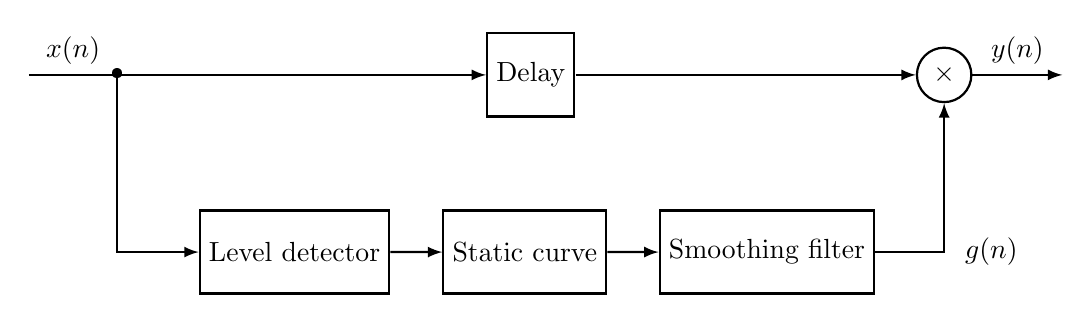
\begin{tikzpicture}[auto, thick, node distance=0.6cm, >=latex, scale = 0.75]
	\draw
	node at (7,0)[delay] (d1) {Delay} 
	node at (14,0)[prod] (p1) {\product}
	node at (3,-3)[delay](d2){Level detector}
	node at (6.9,-3)[delay](d3){Static  curve}
	node at (11,-3)[delay](d4){Smoothing filter}
	node at (14,-3)  (a)[] {} node [right of = a ]{$g(n)$};
	
	\draw[-](-1.5,0) -- node {$x(n)$} (0,0);
	\draw[->](p1) -- node {$y(n)$} (16,0);
	\draw[->](0,0) |- (d2);
	\draw[->](d2) -- (d3);
	\draw[->](d3) -- (d4);
	\draw[->](d4) -| (p1);
	\draw[->](0,0) -- (d1);
	\draw[->](d1) -- (p1);
	\draw node at (0,0) {\textbullet};
	\end{tikzpicture}
	\textbf {Figure} 
\end{center}
The level detector follows one of the two approaches :
\begin{itemize}
\item A full-wave rectifier in combination with an AR-averager with very short attack time may be used to track the peak value of the signal.
\item A square averaged with only a single time-constant provides the RMS value, measuring the signal's power.
\end{itemize}

\begin{center}
	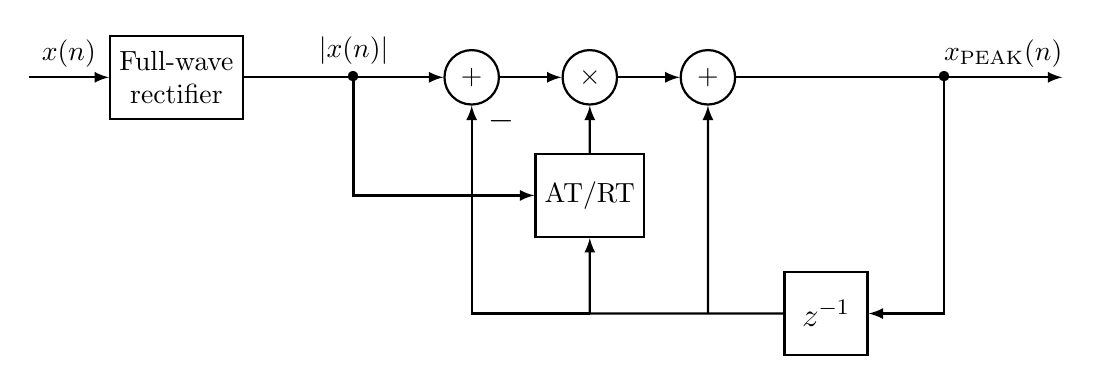
\begin{tikzpicture}[auto, thick, node distance=0.6cm, >=latex, scale = 0.75]
	\draw
	node at (-1,0) [delay,align=center] (d1) {Full-wave \\rectifier}
	node at (2,-0.35) [] (a) {} node [above of = a] {$\left|x(n)\right|$}
	node at (4,0) [sum] (s1) {+}
	node at (6,0) [prod] (p1) {\product}
	node at (8,0) [sum] (s2) {+}
	node at (6,-2) [delay] (d2){AT/RT}
	node at (10,-4) [delay] (d3) {\delay}
	node at (4.5,-0.75) {\large$-$};
	
	\draw[->](-3.5,0)--node {$x(n)$} (d1);
	\draw[->](d1)--(s1);
	\draw[->](s1)--(p1);
	\draw[->](p1)--(s2);
	\draw[->](2,0)|-(d2);
	\draw[->](6,-4)--(d2);
	\draw[->](6,-4)-|(s1);
	\draw[-](6,-4)--(d3);
	\draw[->](8,-4)--(s2);
	\draw[->](d2)--(p1);
	\draw[->](12,0)|-(d3);
	\draw[-](s2)--(12,0);
	\draw[->](12,0)--node {$x_{\mathrm{PEAK}}(n)$}(14,0);
	
	\draw node at (2,0) {\textbullet};
	\draw node at (12,0) {\textbullet};
	
	\end{tikzpicture}
	\textbf {Figure} Peak measurement for a dynamic range controller.
\end{center}
\begin{center}
	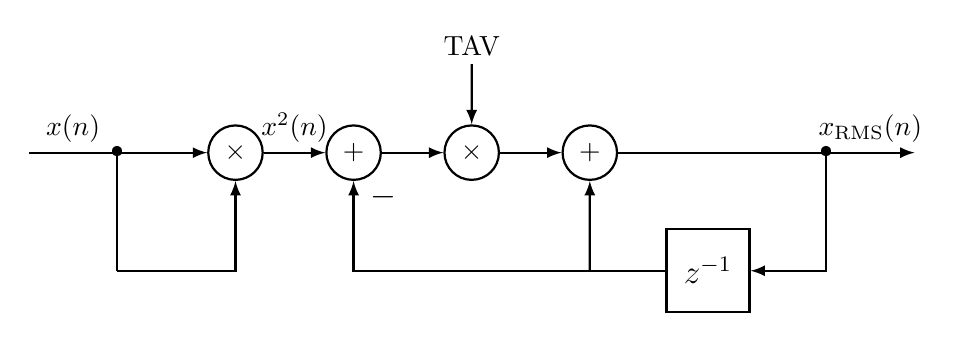
\begin{tikzpicture}[auto, thick, node distance=0.6cm, >=latex, scale = 0.75]
		\draw
		node at (2,0) [prod] (p1) {\product}
		node at (4,0)[sum] (s1) {+}
		node at (6,0) [prod] (p2) {\product}
		node at (8,0) [sum] (s2) {+}
		node at (10,-2) [delay] (d1) {\delay}
		node at (4.5,-0.75){\large$-$}
		node at (6,1.8) {TAV};
		
		\draw[-](-1.5,0)--node {$x(n)$} (0,0);
		\draw[->](0,0)--(p1);
		\draw[-](0,0)--(0,-2);
		\draw[->](0,-2)-|(p1);
		\draw[->](p1)--node{$x^2(n)$}(s1);
		\draw[->](s1)--(p2);
		\draw[->](6,1.5)--(p2);
		\draw[->](d1)-|(s1);
		\draw[->](p2)--(s2);
		\draw[-](s2)--(12,0);
		\draw[->](8,-2)--(s2);
		\draw[->](12,0)--node {$x_{\mathrm{RMS}}(n)$} (13.5,0);
		\draw[->](12,0)|-(d1);
		
		\draw node at (0,0) {\textbullet};
		\draw node at (12,0) {\textbullet};
		
	\end{tikzpicture}
	\textbf {Figure} RMS measurement for a dynamic range controller.
\end{center}
The static curve decides which function(limiter, compressor, expander,\dots) the dynamic range controller emploies. It is best described on a dB scale, so we introduce $X$, $G$ and $Y$ for the levels of the respective signals in dB. The multiplication at the dynamic range controller’s output then becomes $Y = X + G$.\\

The dynamic behavior of a dynamic range controller is influenced by the level measurement approach (with attack AT and release time RT for peak measurement and averaging time TAV for RMS measurement) and further adjusted with a smoothing filter.
\section{Limiter}
The limiter is used to control the highest peaks in the signal, but to otherwise change the dynamics of the signal as little as possible.
\begin{align*}
G &=
\begin{cases} 
0 \ \mbox{dB}  &\mbox{if }X < LT\\
LT-X &\mbox{else}
\end{cases}
\end{align*}
\[
g ( n ) = \min \left( 1 , \frac { l t } { x _ { \mathrm { PEAK } } ( n ) } \right)
\]
\begin{center}
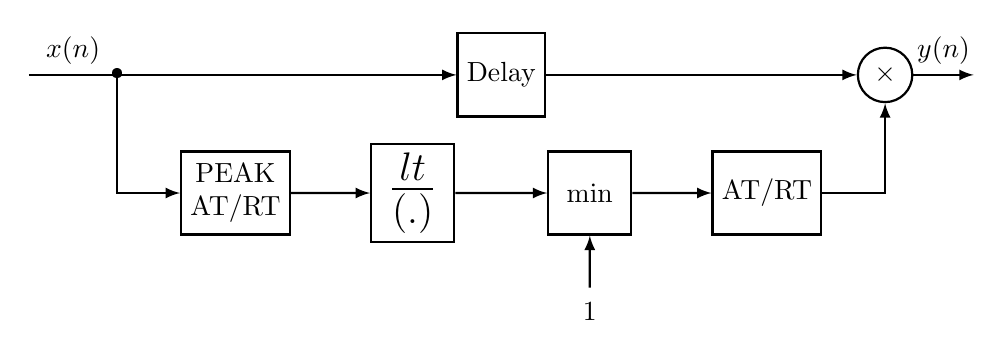
\begin{tikzpicture}[auto, thick, node distance=0.6cm, >=latex, scale = 0.75]
\draw
node at (1,0) {\textbullet}
node at (3,-2) [delay,align=center](d1) {PEAK \\ AT/RT}
node at (6,-2) [delay] (d2){\huge$\frac{lt}{(.)}$}
node at (9,-2) [delay] (d3){min}
node at (12,-2) [delay] (d4){AT/RT}
node at (14,0) [prod] (p1){\product}
node at (7.5,0) [delay] (d5){Delay}
node at (9,-4) {1};

\draw[-](-0.5,0)--node{$x(n)$}(1,0);
\draw[->](1,0)|-(d1);
\draw[->](d1)--(d2);
\draw[->](d2)--(d3);
\draw[->](d3)--(d4);
\draw[->](d4)-|(p1);
\draw[->](1,0)--(d5);
\draw[->](d5)--(p1);
\draw[->](9,-3.6)--(d3);
\draw[->](p1)--node{$y(n)$}(15.5,0);
\end{tikzpicture}
\textbf {Figure} Block diagram of a limiter
\end{center}

\begin{lstlisting}
function y = limiter(x, lt)
% function y = limiter(x, lt)
% Author: Yangang Cao

at = 0.3; % Attack time
rt = 0.01; % Release time
delay = 5;

xpeak = 0; % intialization
g = 1; % gain
buffer = zeros(1,delay);

for n = 1:length(x)
	a = abs(x(n));
	if a > xpeak
		coeff = at;
	else
		coeff = rt;
	end
	xpeak = (1-coeff) * xpeak + coeff * a; % Level detector (A full-wave rectifier in combination with an AR-averager)
	f = min(1, lt/xpeak); %Static curve
	if f < g
		coeff = at;
	else
		coeff = rt;
	end
	g = (1-coeff) * g + coeff * f; % Smoothing filter
	y(n) = g * buffer(end);
	buffer = [x(n) buffer(1:end-1)];
end
\end{lstlisting}
\section{Compressor and Expander}
\begin{align*}
G &=
\begin{cases} 
CS\cdot(CT-X)   &\mbox{if } X>CT \\
0 \ \mbox{dB}  &\mbox{if }ET\leqslant X\leqslant CT\\
ES\cdot(ET-X) &\mbox{if }X<ET
\end{cases}\\
&=min(0, \ CS\cdot(CT-X),\ ES\cdot(ET-X)).
\end{align*}
\begin{center}
	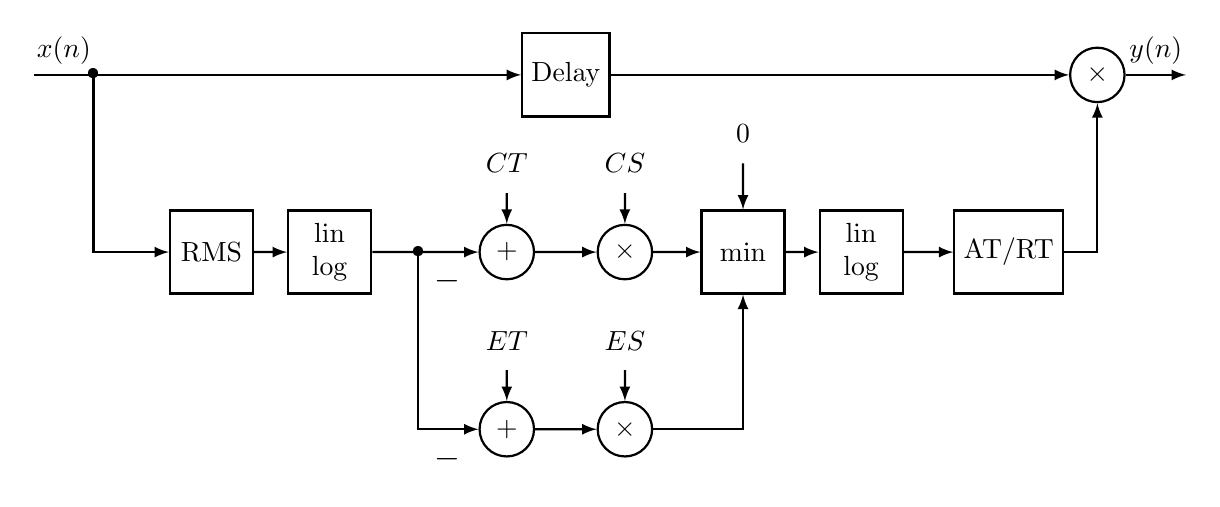
\begin{tikzpicture}[auto, thick, node distance=0.6cm, >=latex,scale = 0.75]
	\draw
	node at (5.5,-3) {\textbullet}
	node at (0,0)  {\textbullet}
	node at (2,-3) [delay] (d1) {RMS}
	node at (4,-3) [delay,align=center] (d2) {lin\\ log}
	node at (7,-3) [sum] (s1) {+}  node at (7,-1.5){$CT$}
	node at (9,-3) [prod] (p1) {\product} node at (9,-1.5){$CS$}
	node at (11,-3) [delay] (d3) {min}
	node at (13,-3) [delay,align=center] (d4) {lin\\ log}
	node at (15.5,-3) [delay] (d5) {AT/RT}
	node at (17,0) [prod] (p3) {\product}
	node at (8,0) [delay] (d6) {Delay}
	node at (7,-6) [sum] (s2) {+} node at (7,-4.5){$ET$}
	node at (9,-6) [prod] (p2) {\product} node at (9,-4.5){$ES$}
	node at (11,-1) {0}
	node at (6,-3.5) {\large$-$}
	node at (6,-6.5){\large$-$}
	;
	\draw[->](0,0)--(d6);
	\draw[->](d6)--(p3);
	\draw[->](0,0)|-(d1);
	\draw[->](d1)--(d2);
	\draw[->](d2)--(s1);
	\draw[->](s1)--(p1);
	\draw[->](p1)--(d3);
	\draw[->](d3)--(d4);
	\draw[->](d4)--(d5);
	\draw[->](d5)-|(p3);
	\draw[->](5.5,-3)|-(s2);
	\draw[->](s2)--(p2);
	\draw[->](p2)-|(d3);
	\draw[->](7,-2)--(s1);
	\draw[->](9,-2)--(p1);
	\draw[->](7,-5)--(s2);
	\draw[->](9,-5)--(p2);
	\draw[->](11,-1.5)--(d3);
	\draw[-](-1,0)--node {$x(n)$} (0,0);
	\draw[->](p3)--node {$y(n)$} (18.5,0);
	\end{tikzpicture}
	\textbf {Figure} Block diagram of a compressor/expander
\end{center}
\[
g ( n ) = \min \left( 1 , \left( \frac { x _ { \mathrm { RMS } } ( n ) } { c t ^ { 2 } } \right) ^ { - C S / 2 } , \left( \frac { x _ { \mathrm { RMS } } ( n ) } { e t ^ { 2 } } \right) ^ { - E S / 2 } \right),
\]
\begin{lstlisting}
function y = compexp(x, CT, CS, ET, ES)

tav = 0.01;
at = 0.03;
rt = 0.003;
delay = 150;

xrms = 0;
g = 1;
buffer = zeros(1,delay);

for n = 1:length(x)
	xrms = (1-tav) * xrms + tav * x(n)^2;
	X = 10*log10(xrms);
	G = min([0, CS * (CT - X), ES * (ET - X)]);
	f = 10^(G/20);
	if f < g
		coeff = at;
	else
		coeff = rt;
	end
	g = (1-coeff) * g + coeff * f;
	y(n) = g * buffer(end);
	buffer = [x(n) buffer(1:end-1)];
end

\end{lstlisting}
\section{Noise Gate}
A noise gate can be considered as an extreme expander with a slope of −∞. This results in the complete muting of signals below the chosen threshold NT. As the name implies, the noise gate is typically used to gate out noise by setting the threshold just above the level of the background noise, such that the gate only opens when a desired signal with a level above the threshold is present. A particular application is found when recording a drum set. Each element of the drum set has a different decay time. When they are not manually damped, their sounds mix together and the result is no longer distinguishable. When each element is processed by a noise gate, every sound can automatically be faded out after the attack part of the sound. This results in an overall cleaner sound.\\
\begin{center}
	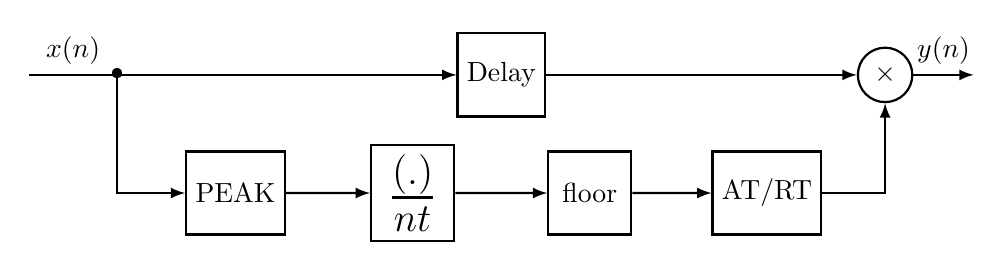
\begin{tikzpicture}[auto, thick, node distance=0.6cm, >=latex, scale = 0.75]
	\draw
	node at (1,0) {\textbullet}
	node at (3,-2) [delay](d1) {PEAK}
	node at (6,-2) [delay] (d2){\huge$\frac{(.)}{nt}$}
	node at (9,-2) [delay] (d3){floor}
	node at (12,-2) [delay] (d4){AT/RT}
	node at (14,0) [prod] (p1){\product}
	node at (7.5,0) [delay] (d5){Delay};

	
	\draw[-](-0.5,0)--node{$x(n)$}(1,0);
	\draw[->](1,0)|-(d1);
	\draw[->](d1)--(d2);
	\draw[->](d2)--(d3);
	\draw[->](d3)--(d4);
	\draw[->](d4)-|(p1);
	\draw[->](1,0)--(d5);
	\draw[->](d5)--(p1);
	\draw[->](p1)--node{$y(n)$}(15.5,0);
	\end{tikzpicture}
	\textbf {Figure} Block diagram of a noise gate
\end{center}

The functional units of a noise gate are shown in Figure 4.16. The decision to activate the gate is typically based on a peak measurement which leads to a fade in/fade out of the gain factor g(n) with appropriate attack and release times. Further possible refinements include the use of two thresholds to realize a hysteresis and a hold time to avoid unpleasant effects when the input level fluctuates around the threshold. These are demonstrated in the implementation given in following code.
\begin{lstlisting}
function y=noisegt(x,holdtime,ltrhold,utrhold,release,attack,a,Fs)

% noise gate with hysteresis
% holdtime: time in seconds the sound level has to be below the 
%		    threshhold value before the gate is activated
% ltrhold: threshold value for activating the gate
% utrhold: threshold value for deactivating the gate > ltrhold
% release: time in seconds before the sound level reaches zero
% attack: time in seconds before the output sound level is the 
%		  same as the input level after deactivating the gate
% a: pole placement of the envelope detecting filter < 1
% Fs: sampling frequency

rel = round(release*Fs);  %number of samples for fade 
att = round(attack*Fs);   %number of samples for fade 
g = zeros(size(x));
lthcnt = 0;
uthcnt = 0;
ht = round(holdtime*Fs);
h = filter([(1-a)^2], [1.0000 -2*a a^2], abs(x)); %envelope detection 
h = h / max(h);
for i = 1: length(h)
	if (h(i) <= ltrhold) | ((h(i) < utrhold) & (lthcnt > 0)) % Value below the lower threshold?
		lthcnt = lthcnt + 1;		
		uthcnt = 0;
		if lthcnt > ht % Time below the lower threshold longer than the hold time?
			if lthcnt > (rel + ht) 
				g(i) = 0;
			else
				g(i) = 1 - (lthcnt-ht) / rel;		% fades the signal to zero
			end;
		elseif ((i < ht) & (lthcnt == i))
			g(i) = 0;
		else
			g(i) = 1;
		end;
	elseif (h(i) >= utrhold) | ((h(i) > ltrhold) & (uthcnt > 0))	
	% Value above the upper threshold or is the signal being faded in?
		uthcnt = uthcnt + 1;
		if (g(i-1) < 1) % Has the gate been activated or isn't the signal faded in yet?
			g(i) = max(uthcnt/att, g(i-1));
		else
			g(i) = 1;
		end;
		lthcnt = 0;
	else
		g(i) = g(i-1);
		lthcnt = 0;
		uthcnt = 0;
	end; 
end;
y = x .* g;
y = y * max(abs(x)) / max(abs(y));

\end{lstlisting}
\end{document}
